\begin{figure*}[t!]
    \begin{subfigure}[t]{0.48\textwidth}
        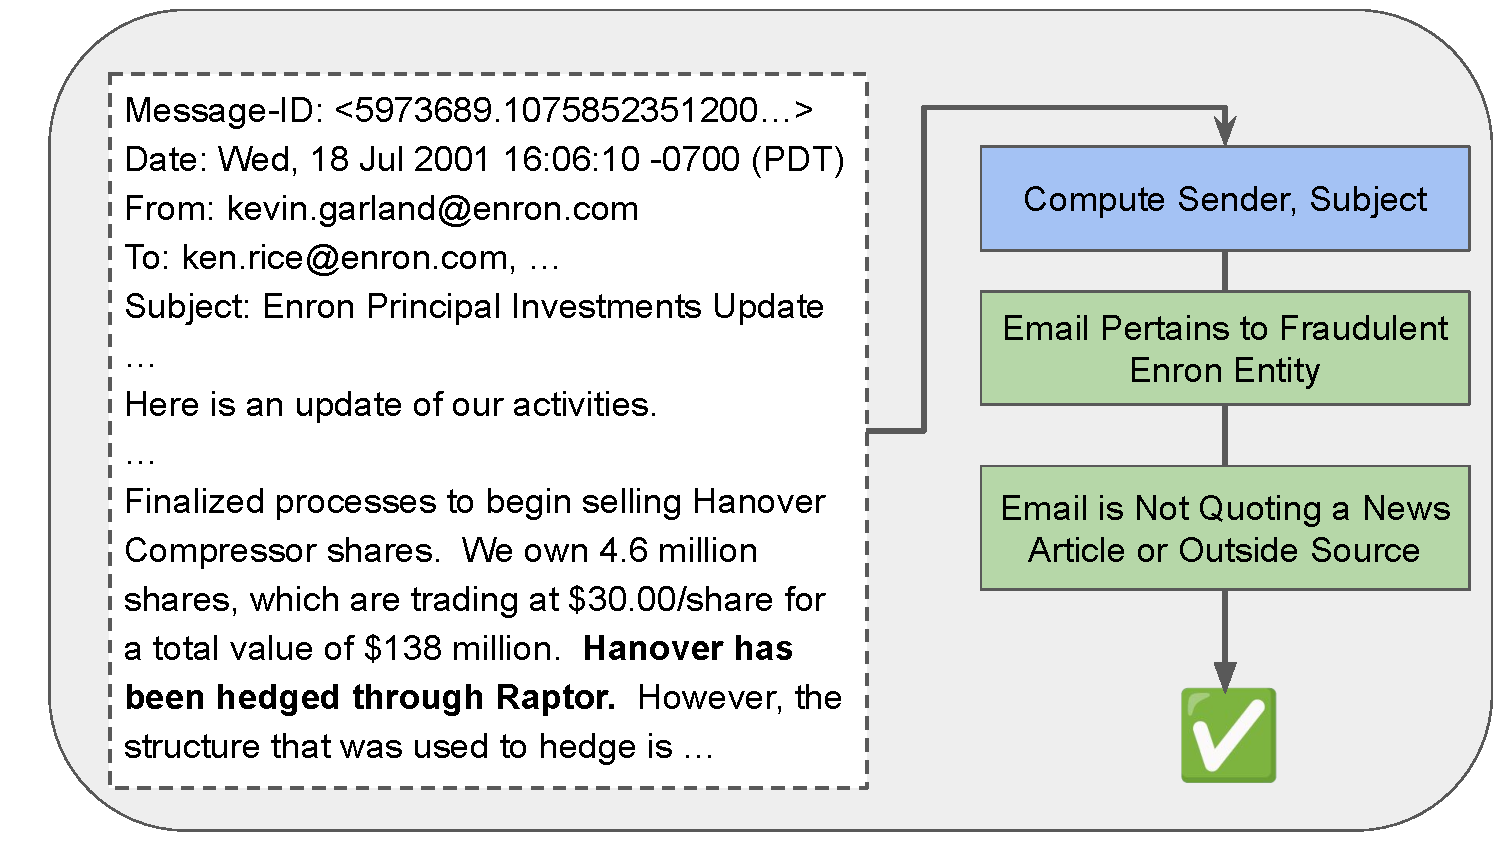
\includegraphics[width=\textwidth]{imgs/PZ-DIAGRAMS-enron-good.pdf}
        \caption{Example of a positive entry in the Legal Discovery workload. This email meets the criteria of (1) mentioning a fraudulent entity (in this case, ``Raptor") and (2) not quoting from a news article or a source outside of Enron.}
    \label{fig:legal-discovery-correct}
    \end{subfigure}
    \hfill
    \begin{subfigure}[t]{0.48\textwidth}
        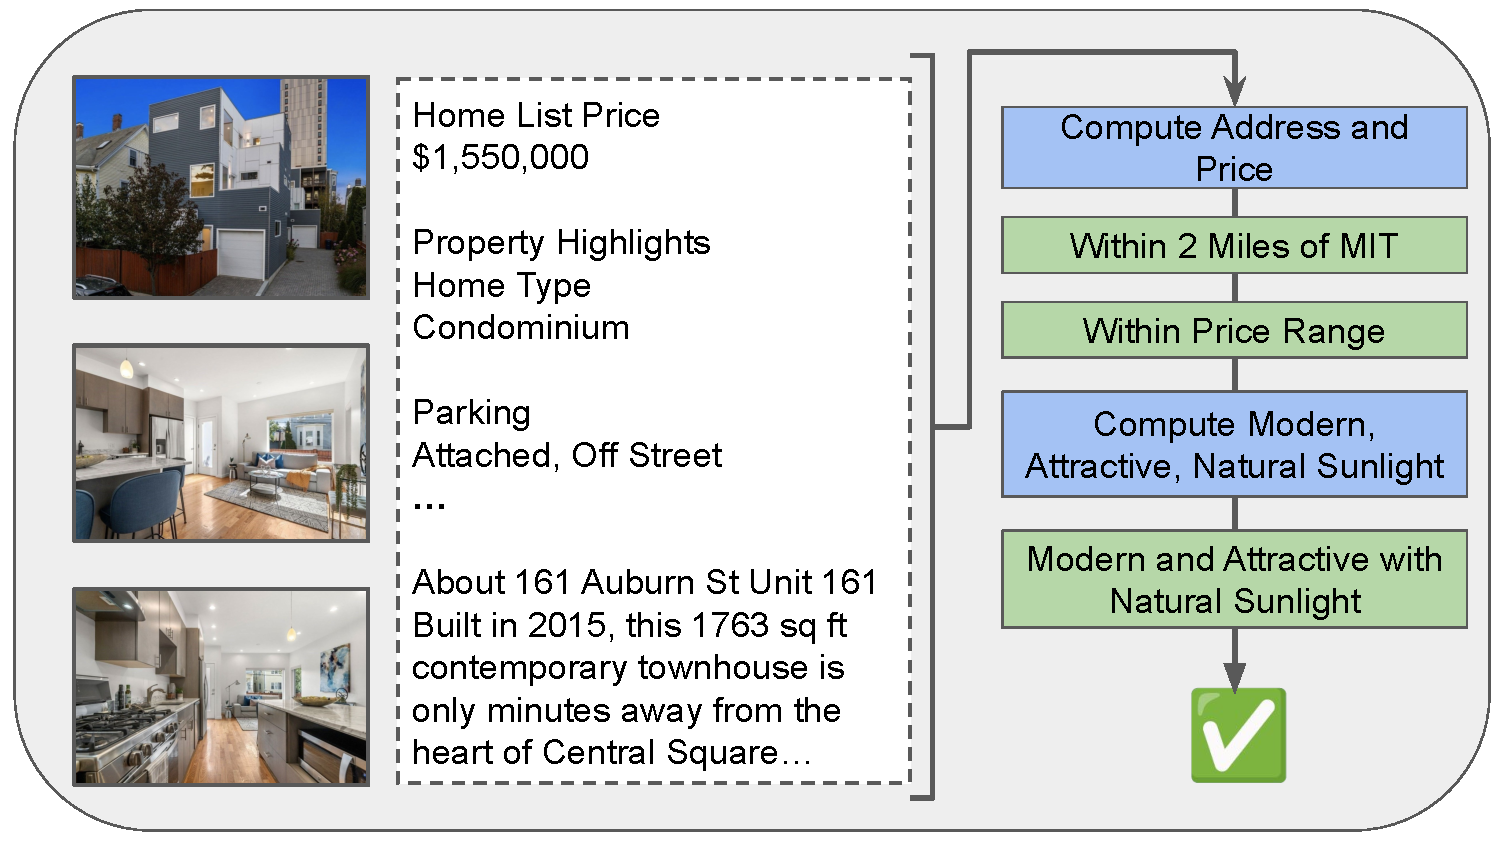
\includegraphics[width=\textwidth]{imgs/PZ-DIAGRAMS-real-estate-good.pdf}
        \caption{Example of a positive entry in the Real Estate Search workload. The house meets the three criteria of being (1) close to MIT (2) within the user's price range and (3) modern and attractive with lots of natural sunlight.}
    \label{fig:real-estate-search-correct}
    \end{subfigure}
    \centering
    \begin{subfigure}[b]{0.95\textwidth}
        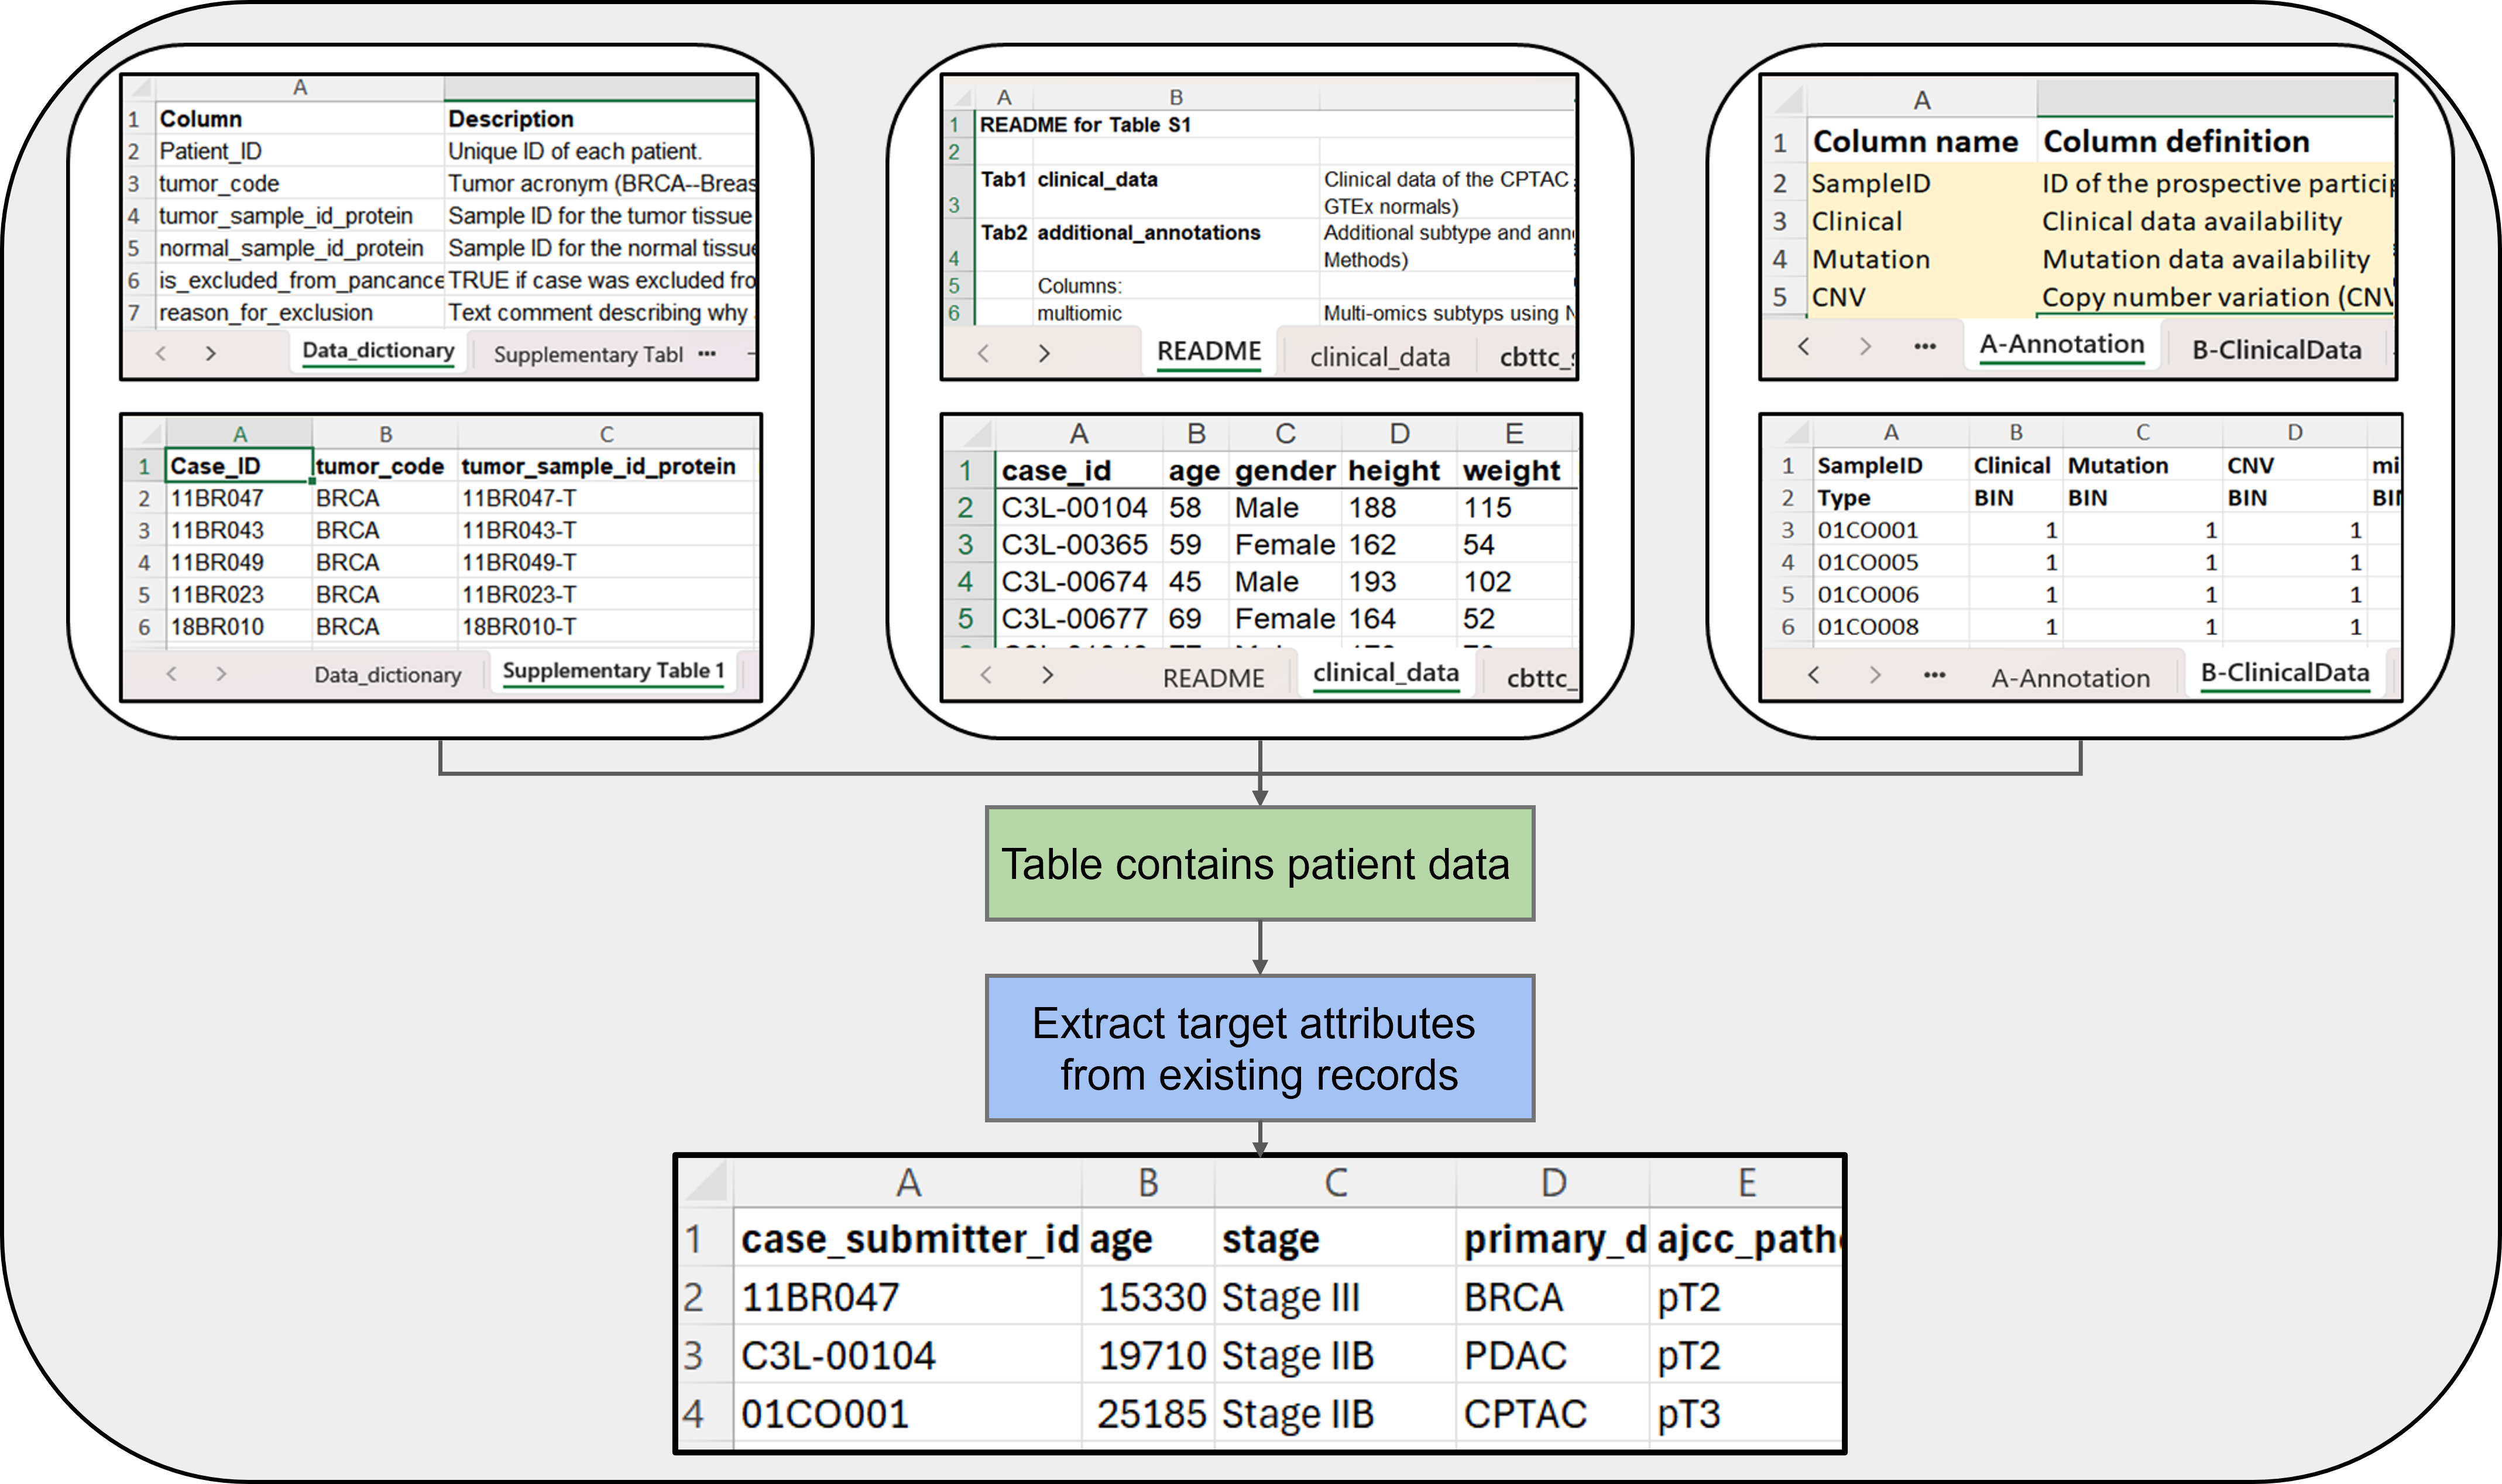
\includegraphics[width=\textwidth]{imgs/biofabric_matching.png}
        \caption{Example of the Medical Schema Matching workload. Three spreadsheets contain several tables and \system{} (1) filters for tables that relate to patient data and (2) matches and extracts the relevant attributes, consolidating a single table with a target schema.}
        \label{fig:biofabric-matching}
    \end{subfigure}
    \caption{Positive examples from the Legal Discovery and Real Estate Search workloads, as well as an overview of the Medical Schema Matching workload. Negative examples can be found in the Appendix (\autoref{fig:negative-examples}).}
    \label{fig:workloads}
\end{figure*}


Before we describe the details of the \system{} system, it is useful to discuss the workloads \system{} aims to support, in particular the SAPP workloads.

As discussed in \autoref{sec:intro}, SAPPs (1) combine traditional data processing and AI elements, (2) potentially process large amounts of data, and (3) can be decomposed into a tree of operations over sets of data objects. As a running example, consider the Real Estate Search task in \autoref{fig:real-estate-search-correct}. In this task, the user wants to search all of the real estate listings near Cambridge, MA to find a house that is (a) modern and attractive, (b) within two miles of MIT, and (c) within the user's price range.

This task clearly satisfies the first criterion: determining whether a house is ``modern and attractive" likely requires using some vision or text model to process the textual listings and images. Moreover, depending on the dataset, recovering price and location data may require extraction from text.  The second criterion is satisfied because --- as of this writing --- Zillow shows 1,327 listings for homes in the Cambridge and Boston areas, and each listing contains a text description along with (typically) 10 or more images. As for the third criterion, the query clearly has a set of objects as both input and output. It is easy to see how we might first have an operator that extracts price and location fields from the raw data, then a second that applies traditional selection predicates. Finally, the system might have an operator that extracts whether the images show a "modern and attractive" residence.  \autoref{fig:real-estate-search-correct} shows a conceptual pipeline, with imperative steps listed in blue, satisfied logical tests in green, and failed logical tests in red.

{\bf Optimization Challenges.} The ideal implementation of an AI system for a SAPP workload will jointly optimize its AI- and conventional data processing elements. For example, in Real Estate Search, an extremely naive implementation might waste time and money processing images of apartments to test whether they are ``modern and attractive" --- only to discard them when they fail to meet conventional constraints. A slightly more sophisticated implementation would reorder the plan so that it applies the restrictive conventional constraints first, thereby avoiding the time and expense of invoking a vision model on candidates that will later be discarded. Further optimizations might process the text description first to evaluate whether an apartment is likely to be ``modern and attractive", and then apply an image processing method only when deemed necessary. The decisions around which optimizations to use and when to use them will have to be made for each new task and dataset.

% Figure~\ref{fig:biofabric-matching} shows data and operations for the Medical Schema Matching task. In this case, the user wants to (a) filter input spreadsheet tabs to retain only those tables that contain patient data, and (b) integrate the surviving tables' schemas.  This task satisfies the scale criterion for SAPPs: we can have dozens of source papers, and each source paper can have dozens of associated datasets. Solving it entails processing AI tasks (such as filtering based on table content and schema integration) and straightforward data loading steps.  Satisfied logical constraints are in green, and computational steps are in blue.

At its core, optimizing an AI system to execute a given SAPP workload requires making accurate predictions about the runtime, cost, and quality of each semantic and conventional data processing step. Estimating these metrics for semantic tasks can be particularly challenging. For example, estimating the runtime and cost for a vision model requires knowing the average number of input and output tokens per record as well as the total number of records that will be processed by the model (i.e., its cardinality). Estimating the quality of an output --- especially without labelled data --- may require using heuristics that can be error prone, or comparing against an expensive "champion" model. Finally, for every physical optimization available to the system (such as using an ensemble of vision models or decreasing the image resolution), the optimizer needs to predict the optimization's impact on these metrics.

%  If this operation follows one or more filters, computing its cardinality would require knowing the fraction of records filtered upstream (i.e., knowing the upstream filters' selectivity).

% The ideal SAPP implementation will jointly optimize the semantic and conventional elements. For example, in the investment hypothesis application, a naive implementation might spend a lot of time generating candidates in the semantic search phase, only to throw them all away because none of them meet the conventional constraints.  A more sophisticated implementation would reorder the plan so that it applies the restrictive conventional constraints first, and thereby avoid the time and expense of generating candidates that will be discarded.
% \tim{A predicate pushdown is almost too simple. From all the examples above I would argue: do (a) first traditional operators followed by (b) LLM operators. And then use some standard tuning things for the LLM operator (e.g., model selection or prompt tuning. Do you have an example, which goes beyond that vanilla optimizaion. Something which shows that it is a complex trade=off and a declarative approach is really needed. }

{\bf System Design Challenges.} An ideal system for processing SAPP workloads will also require minimal engineering effort to maintain application code over time, in the face of changing user needs and input data. To the extent that AI components have been integrated into data applications in the past, significant effort went into training models narrowly tailored for a particular semantic task. Outside of a few tech giants, models were infrequently retrained. Models were restrictive enough that the space of system-wide performance tuning decisions was not large, and at any rate models changed infrequently enough that system-wide tuning did not have to happen often.

The modern AI landscape has changed all of these assumptions. The set of models and adjacent AI approaches (such as prompting strategy) is large and rapidly changing. The space of system-wide performance decisions is vast, and the best decision changes with each new model, task, business need, and dataset. Anecdotally, we have heard several RAG users and vendors start to complain that deploying these systems requires making repeated configuration decisions that reflect reasonable performance vs quality trade-offs; this is a task that traditional data administrators are often not equipped to make. \system{} aims to enable AI system engineers to focus on programming the system logic while letting the optimizer select which models and physical optimizations are needed to meet the user's preferences for cost, runtime, or data quality.
%\tim{I get and really like the idea, but I think you need to support it with better examples}

%and tuning the rest of the AI system to ensure acceptable performance. Small changes to the input data (e.g., adding a new source of information) or business needs (e.g., improving recall at fixed cost) would require re-training and re-tuning many pieces of the system. \system{} enables AI system engineers to focus on programming the system logic while letting the optimizer select which models and physical optimizations are needed to meet the user's policy preference(s) (such as minimizing cost).

% Like any applications that use model outputs, AI systems for SAPP workloads may benefit from user feedback and fine-tuning. However, SAPPs' layers of operations make implementing this feedback loop enormously more complex: a particular model output may need to be tracked through multiple rounds of data processing so that the user's thumbs-up/thumbs-down vote can be used to improve the right model in the execution tree. However, if the AI system is implemented inside the \system{} system, tracking user feedback signals can be done automatically, and \system{} can automatically fine-tune underlying models when appropriate. Moreover, AI systems that alternate between quality adjustment and deployment phases can be easily supported by \system's re-optimization capabilities.

%Retrieval Augmented Generation (RAG) applications were probably the first widely-identified workload in this area. These applications usually involve two steps: (1) query relevance retrieval of conventionally-produced documents, followed by (2) AI production of a user-consumable result that is driven by the fetched documents. Even this dead-simple architecture exhibits performance, cost, and quality tradeoffs when the system designer decides how many documents to fetch from a vector database in Step 1. Too few means the LLM may not have relevant information it needs, while too many means the system performs unnecessary queries.

% Another use case lies in answering analytical queries over heterogeneous data, often found in a data lake, and often using information extraction~\cite{arora2023language, shin2015incremental, DBLP:conf/webdb/CafarellaSE07, DBLP:conf/vldb/ChuBCDN07}. These {\em semantic analytical applications} --- or, \textbf{SAPPs} --- frequently require interleaved data acquisition steps, conventional analytical queries, and AI operations. The AI operations process unstructured data, require broad domain knowledge to implement, or have loose specifications that users may not be able to specify more completely. Performance, cost, and quality tradeoffs are likely to be common. Some data management tasks, such as data integration, may also fall into this category if they primarily exist for answering analytical questions.


%
\subsection{Additional Workloads}
% \matt{While SAPPs are an exciting new class of AI workloads which \system{} is designed to support, it also helps users optimize more ``traditional" systems such as ones using Retrieval Augmented Generation (RAG).}
Beyond SAPPs, there are a number of workloads which \system{} is well-suited to implement given its relational model and optimizer.

\noindent {\bf Document-driven discovery.} Organizations and individuals often wish to extract insights from sets of documents. For example, investors may wish to examine the footnotes of public US banks' SEC filings to see if they are at risk of a liquidation event. As another example, database researchers may try to process five years of VLDB and SIGMOD papers to extract specific metadata of interest (e.g., how the number of figures in accepted papers has varied over time).
\mjf{why isn't this a SAPP?  Seems to meet all the criteria}

Such tasks can easily be performed using \system{}. As shown previously in \autoref{fig:email} and \autoref{fig:examples}, users simply provide their source documents as an input {\tt Dataset} and define the metadata they wish to extract using their own {\tt Schema}. They may also perform additional post-processing on the extracted metadata following the schema conversion.

\noindent {\bf Multimodal integration.} Users often wish to integrate multiple datasources of differing modalities in order to enhance their ability to extract quantitative insights. For example, an insurance company may collect photos of a car crash along with police reports to help determine whether the driver they insure is at fault or not. Similarly, firefighters may collect streaming video data along with live weather maps to try to pinpoint the location of a brush fire. Once again, \system{} can assist users with creating AI systems for such workloads by allowing users to write simple {\tt Schemas} against each data modality to extract quantitative fields of interest.

\noindent {\bf Schema matching.}
To manage large collections of structured data from different sources often requires matching schemata across different tables.
For example, a medical researcher may wish to perform a large-scale study that requires integrating new patient data collected by previous field studies together with new experimental observations.
Or, environmental scientists may want to analyze climate change using historical data collected with different sensors across different geographical regions.
With the use of \system{}, users can write a simple specification of the target {\tt Schema} using natural language, and let \system{} automatically infer how to extract and match the existing attributes from all source datasets.

\noindent {\bf RAG systems.} The Retrieval Augmented Generation (RAG) architecture has rapidly become a first-class use case for neural models in enterprise settings. They are characterized by a two-stage process: first, a retrieval model is used to identify a set of candidate input documents, and then a generation model is used to produce a high-quality output based on the inputs. Even this dead-simple architecture exhibits performance, cost, and quality tradeoffs when the system designer decides how many documents to fetch from a vector database in Step 1. Too few means the LLM may not have relevant information it needs, while too many means the system performs unnecessary queries. \matt{\system{} is designed to optimize for these types of tradeoffs, thus supporting RAG applications is quite natural.}

\tim{I find it confusing that you mention RAG here. Everything else are use cases, RAG is a technique to achieve a particular goal, e.g., schema matching. For me it is on the same level as model selection, code generation, etc,. which are all tools/techniques to achieve a specific goal.} 
\mjf{I also think the above examples except for RAG could be considered SAPPs - no?  If so, then it is indeed interesting that the system (or at least the insights underlying it) could be used to support RAG, which as Tim says, seems different from the others.}

\system\ is designed to use the RAG architecture in two different ways. First, it can employ RAG-style methods as part of its query plan. For example, consider \st{a topic summarization program in \autoref{fig:extraction-example}} the use case of topic summarization over a set of documents. If the input document is larger than any available model's maximum token size, \system\ can decide, during synthesis of the convert operation, to use a RAG-style method to make the subtask manageable. That is, it may: (1) decompose the input text into smaller chunks, (2) choose chunks that are both relevant and will fit in the model's context size, then (3) generate the output summary using the selected chunks. This is a purely "internal" RAG approach, which is invisible to the user.

\matt{Matt: Re-reading the paragraph above made me realize that it pretty much summarizes Chunwei's input token reduction technique, because I doubt 95\% of users have documents which cannot fit in the context of the newest models. The more I think about it, the more I understand Tim's comment that, at least in our worldview, RAG is a token-reduction optimization which has quality and runtime tradeoffs as well. The key point we want to make is that PZ can optimize your RAG system for you --- but I think that falls outside of ``workloads" and maybe this text should go into ``optimizations"? Perhaps we should reframe this subsection as illustrating how ``traditional workloads" can be represented as SAPPs. I.e. ``document-driven discovery is a SAPP where the input is ... multimodal integration is a SAPP which focuses on the extraction of structured fields from ... Schema matching is a SAPP in which ..." }

The system can also support "external" RAG applications in which the user has an external data store of documents. \system\ allows users to define their own datasources, and can use these sources as part of the query plan. We understand from talking with industrial contacts that one of the primary engineering challenges encountered when building RAG systems is managing the inevitable quality/runtime tradeoffs. For example, how many 
documents should be returned by the vector database in response to a query? Too many, and the system is unnecessarily slow; too few, and the system yields bad results. This kind of tradeoff is exactly what \system\ was designed to handle: we are currently working on an extension that will allow \system\ to optimize these external RAG database queries.

% \noindent {\bf Database Administration}


% Older content:

% \noindent {\bf }

% Functionalities we wish to highlight:
% \begin{itemize}
%     \item \textbf{Queries over text / PDFs}
%     \begin{itemize}
%         \item Searching Enron emails for ref. to Special Purpose Entities (SPEs) (i.e. fraud)
%         \item Matching investment hypothesis to companies' public filings
%     \end{itemize}
%     \item \textbf{Queries over images}
%     \begin{itemize}
%         \item Semantic search over image repos (``find a photo of my dog playing in the snow")
%         \item Satellite image classification (Amazon deforestation)
%         \item Stream classifiers (e.g. imagine having an Amber Alert which only requires updating the Alert prompt rather than re-training an image classifier)
%     \end{itemize}
%     \item \textbf{Multi-modal queries}
%     \begin{itemize}
%         \item Fake Amazon products \& reviews
%         \item Search over video / audio + transcription
%         \item Investment hypothesis (PDF + stock time-series data)
%     \end{itemize}
%     \item \textbf{Queries which require using RAG}
%     \begin{itemize}
%         \item Understanding my tax liability (querying IRS docs + tax law)
%         \item (Possibly investment hypothesis example; we may need to pre-process PDFs and perform RAG over their contents)
%     \end{itemize}
% \end{itemize}